\newpage

\section{Simulation Analysis}
\label{sec:simulation}

The basic template for a converter circuit is as follows:

\begin{figure}[H]
        \centering
        \includegraphics[width=\textwidth, trim = 0 4cm 0 4cm, clip]{acdc.pdf}
        \caption{Template}
        \label{acdc}
\end{figure}

\subsection{Envelope Detector}

An Envelope Detector is comprised of a rectifier and a capacitor.

The rectifier can be either a half-wave rectifier or a full-wave rectifier. A half-wave rectifier only allows for the transfer of positive voltage, therefore resulting in null voltage if the input voltage is negative. The full-wave rectifier allows for the transfer of the absolute value of the voltage. For our circuit, we decided to employ a full-wave rectifier, so as to have as small a gap as possible between peaks in the voltage, and therefore make it easier to even out later in the circuit.

\begin{figure}[H]
        \centering
        \includegraphics[width=0.6\textwidth, trim = 0 4cm 0 2cm, clip]{rectifier.pdf}
        \caption{Full-wave rectifier}
        \label{rectifier}
\end{figure}

We now have the module of the initial signal. In order to start bridging the oscillations, a capacitor is placed next to the rectifier, which discharges as the voltage drops, therefore bridging some of the gap.

\begin{figure}[H]
        \centering
        \includegraphics[width=0.6\textwidth, trim = 0 4cm 0 4cm, clip]{envelope.pdf}
        \caption{Envelope Detector}
        \label{envelope}
\end{figure}

\subsection{Voltage Regulator}

The purpose of the Voltage Regulador is, as the name suggests, to limit the voltage output. One such circuit is as follows:

\begin{figure}[H]
        \centering
        \includegraphics[width=0.6\textwidth, trim = 0 5cm 0 5cm, clip]{regulator.pdf}
        \caption{Voltage Regulator}
        \label{envelope}
\end{figure}

It is known that:

\begin{equation}
        v_O \leq N V_{ON}
        \label{max}
\end{equation}

By performing incremental analysis (that is, saying that each diode is equivalent to a resistor $r_d$):

\begin{equation}
        v_o = \frac{N\;r_d}{N\;r_d + R} v_i
        \label{vo}
\end{equation}

%em baixo, onde está N\;r_d, estava n\;r_d. Corrigi, penso que era suposto ser N
This implies that, if $R$ is much greater than $N\;r_d$, then the amplitude of $v_o$ (AC signal) is almost null, which is our goal. However, this must be balanced with the cost, as resistors are expensive (diodes, on the other hand, are not, so as many as needed may be added to cap $v_o$ at around 12V).

\subsection{Final result}

Combining the envelope detector and the voltage regulator, our circuit is as follows:

\begin{figure}[H]
        \centering
        \includegraphics[width=\textwidth, trim = 2cm 4cm 2cm 4cm, clip]{acdc_ours.pdf}
        \caption{Our template}
        \label{acdc_ours}
\end{figure}

By a lengthy process of trial and error, attempting to maximize the merit figure gave us the following parameters:

\begin{table}[H]
        \centering
        \begin{tabular}{|c|c|}
        \hline
        Parameter & Value \\
        \hline
        \input{../sim/parameters}
        \hline
        \end{tabular}
        \caption{Parameters}
        \label{param}
\end{table}

Following this are shown the time evolution outputs for the Envelope Detector and Voltage Regulator Circuit and also the ripple in $v_o$. 

\begin{figure}[H]
        \centering
        \includegraphics[width=0.6\textwidth, trim = 0 0 0 0, clip]{trans.eps}
        \caption{Simulation results for the Envelope Detector (v2) and Voltage Regulator Circuit (v3) outputs}
        \label{sim_res}
\end{figure}

\begin{figure}[H]
        \centering
        \includegraphics[width=0.6\textwidth, trim = 0 0 0 0, clip]{final.eps}
        \caption{Ripple evolution $(v_0-12)$}
        \label{sim_ripple_res}
\end{figure}
